% Springer Nature Journal Submission Manuscript
% Template: sn-jnl.cls (Springer Nature, 2024/2026)
% Document Class: pdflatex, sn-mathphys-num
\documentclass[pdflatex,sn-mathphys-num,twocolumn]{sn-jnl}
\makeatletter\def\Gm@warning#1{}\makeatother
\usepackage[T1]{fontenc}
\usepackage[utf8]{inputenc}

\usepackage{graphicx}
\usepackage{multirow}
\usepackage{amsmath,amssymb,amsfonts}
\usepackage{amsthm}
\usepackage{mathrsfs}
\usepackage[title]{appendix}
\usepackage{xcolor}
\usepackage{float}
\usepackage{geometry}
\geometry{top=2cm, bottom=2cm, left=1.2cm, right=1.2cm, columnsep=0.65cm}
\definecolor{crimson}{RGB}{180, 20, 20}
\usepackage{textcomp}
\usepackage{manyfoot}
\usepackage{booktabs}
%\usepackage{algorithm}
%\usepackage{algorithmicx}
%\usepackage{algpseudocode}
%\usepackage{listings}
\usepackage{tabularx}
\usepackage{array}

\theoremstyle{thmstyleone}
\newtheorem{theorem}{Theorem}
\newtheorem{proposition}[theorem]{Proposition}

\theoremstyle{thmstyletwo}
\newtheorem{example}{Example}
\newtheorem{remark}{Remark}

\theoremstyle{thmstylethree}
\newtheorem{definition}{Definition}

\raggedbottom


\makeatletter
\setcounter{topnumber}{8}
\setcounter{bottomnumber}{8}
\setcounter{totalnumber}{10}
\setcounter{dbltopnumber}{3}
\renewcommand{\topfraction}{0.98}
\renewcommand{\bottomfraction}{0.98}
\renewcommand{\dbltopfraction}{0.98}
\renewcommand{\textfraction}{0.02}
\renewcommand{\floatpagefraction}{0.85}
\renewcommand{\dblfloatpagefraction}{0.85}
\makeatother

\begin{document}

\title[Economics-Informed ML for Corporate Financial Distress Prediction]{Economics-Informed Machine Learning for Corporate Financial Distress Prediction in Emerging Markets: Monotonic Structural Regularization, Forensic Panel Sanitization, and Out-of-Time Crisis Generalization}

\author*[1]{\fnm{Research} \sur{Team}}\email{corresponding.author@university.edu}

\affil*[1]{\orgdiv{Department of Finance and Computational Intelligence}, \orgname{Advanced Financial Research Institute}, \orgaddress{\city{Hanoi}, \country{Vietnam}}}

\abstract{
Corporate financial distress prediction is a cornerstone of empirical corporate finance and credit risk management. While high-capacity machine learning (ML) classifiers---such as gradient-boosted decision trees (GBDTs) and deep multilayer perceptrons (MLPs)---regularly surpass classical linear scoring models on tabular accounting panels, they suffer from two structural vulnerabilities that impede regulatory adoption in emerging markets. First, unconstrained non-linear estimators fit spurious, non-monotonic relationships in noisy accounting ratios, generating counter-intuitive comparative statics (e.g., predicting lower default probability when leverage increases) and violating structural solvency boundaries. Second, empirical corporate distress studies frequently suffer from severe methodological look-ahead bias arising from random $K$-fold cross-validation across panel years, full-sample winsorization and imputation, unisolated pre-IPO historical backfilling, and survivorship bias when distressed issuers delist. To resolve both challenges simultaneously, we propose an Economically-Informed Machine Learning (EIML) framework comprising two complementary tracks: (i) a tree-based Monotonic GBDT with split-level directional sign constraints, and (ii) a differentiable Economically-Informed Neural Network (EINN) that enforces partial monotonicity via softplus weight reparameterization alongside structural boundary regularization inspired by Merton's contingent-claims theory and Altman's insolvency zone. Evaluated on a forensically audited 15-year panel of 11,455 raw firm-year records (7,602 post-listing transition pairs across 692 non-financial firms listed on HOSE, HNX, and UPCOM from 2008 to 2022) under a zero-look-ahead out-of-time protocol covering the 2021--2022 Vietnamese corporate bond and regulatory delisting crisis ($N_{\text{test}}=2,083$), our EIML framework achieves state-of-the-art discrimination while eliminating economic axiom violations. Under strict 1-year-ahead forward distress transitions ($Y_{i,t+1}^{\text{fwd}}$), Monotonic GBDT attains an out-of-time ROC-AUC of $0.8021$, PR-AUC of $0.3793$, Brier score of $0.0798$, and an Economic Consistency Score (ECS) of $99.97\%$, while Proposed EINN improves PR-AUC by $+4.96\%$ over an unconstrained MLP ($0.3517$ vs.\ $0.3021$) and elevates ECS from $29.00\%$ to $100.00\%$ ($0.00\%$ monotonicity and boundary violations). Under persistent multi-period distress ($Y_{i,t+1}^{\text{ovl}}$), Monotonic GBDT and Proposed EINN achieve ROC-AUCs of $0.9648$ and $0.9592$ with $100.00\%$ economic consistency, successfully flagging major 2022 crisis defaulters (\texttt{FLC}, \texttt{HAI}, \texttt{BII}, \texttt{AMD}, \texttt{GAB}, and \texttt{VKC}) one fiscal year ahead of collapse.
}

\keywords{Corporate Financial Distress Prediction, Economically-Informed Machine Learning, Monotonic Neural Networks, Structural Credit Risk, Look-Ahead Bias, Vietnamese Listed Firms}

\pacs[JEL Classification]{C45, C52, C53, G17, G32, G33}
\pacs[MSC Classification]{68T05, 91B70, 62P05}

\maketitle


\section{Introduction}
\label{sec:intro}

The accurate, timely, and economically interpretable prediction of corporate financial distress is of paramount importance to commercial banks, bondholders, prudential supervisors, and equity investors \citep{beaver1966financial,altman1968financial,campbell2008search}. In emerging capital markets, where institutional disclosure enforcement is evolving, credit ratings coverage is sparse, and corporate borrowing is heavily skewed toward short-term bank credit and privately placed corporate bonds, sudden waves of corporate insolvency can trigger systemic liquidity freezes \citep{altman1995emerging,pham2018financial,tran2023examining}. This vulnerability was starkly illustrated during the 2021--2022 Vietnamese corporate bond and real estate liquidity crisis, when aggressive short-term leverage expansion and weak operating interest coverage culminated in high-profile bond defaults, regulatory trading suspensions, and forced delistings across the Ho Chi Minh Stock Exchange (HOSE) and Hanoi Stock Exchange (HNX).

Historically, the academic literature on corporate default prediction has evolved along two methodological paradigms. The first paradigm comprises classical statistical and structural credit risk models, beginning with univariate ratio analysis \citep{beaver1966financial}, multivariate discriminant analysis ($Z$-score and $Z''$-score) \citep{altman1968financial,altman1995emerging,altman2017financial}, conditional logit and probit models \citep{ohlson1980financial,zmijewski1984methodological}, discrete-time multi-period hazard models \citep{shumway2001forecasting,chava2004bankruptcy,campbell2008search,bauer2014are}, and option-theoretic structural distance-to-default models rooted in \citet{merton1974pricing} \citep{hillegeist2004assessing,duffie2007multi,bharath2008forecasting}. Because these models impose strict parametric functional forms and clear comparative statics, they satisfy regulatory auditability requirements; however, their linear additive specifications cannot capture complex, non-linear interactions among leverage maturity structure, working capital depletion, and operating cash flow coverage.

The second paradigm leverages non-parametric machine learning (ML) and deep learning classifiers---including random forests \citep{breiman2001random}, gradient-boosted decision trees \citep{chen2016xgboost,ke2017lightgbm,prokhorenkova2018catboost}, support vector machines, and deep neural networks \citep{lessmann2015benchmarking,zieba2016ensemble,barboza2017machine,mai2019deep,hosaka2019bankruptcy,gunnarsson2021deep}. While high-capacity ML ensembles consistently achieve superior out-of-sample ranking accuracy on corporate bankruptcy benchmarks, they introduce a fundamental tension between predictive flexibility and economic rationality \citep{bussmann2021explainable,bucker2022transparency,dumitrescu2022machine}. When trained on noisy, heavy-tailed emerging-market accounting panels, unconstrained ML models frequently violate foundational corporate finance axioms. Specifically, an unconstrained multilayer perceptron (MLP) or radial basis function support vector machine (RBF-SVM) can fit local polynomial oscillations where a ceteris paribus increase in total leverage ($\text{Debt}/\text{Assets}$) or short-term debt concentration ($\text{ShortDebt}/\text{TotalDebt}$) counter-intuitively \textit{reduces} predicted default probability. Moreover, in out-of-distribution tail regimes, unconstrained classifiers frequently assign high distress probabilities to nearly debt-free, profitable firms (violating Merton's zero-debt safety boundary) or low distress probabilities to technically insolvent firms with negative equity.

Compounding this modeling challenge is a pervasive methodological flaw in empirical financial ML studies: \textit{look-ahead bias} (information leakage) and inadequate forensic panel hygiene \citep{bailey2014pseudo,lopez2018advances}. A critical audit of recent emerging-market and Vietnamese financial distress studies \citep[e.g.,][]{pham2018financial,vo2019corporate,tran2022explainable,tran2023examining,vu2023lasso} reveals four recurring sources of leakage and distortion:
\begin{enumerate}
    \item \textbf{Cross-sectional random splitting and synthetic oversampling across time:} Applying random $K$-fold cross-validation or random $70/30$ train-test splits (often combined with full-sample SMOTE) across multi-year panel data allows observations from year $t+k$ to inform predictions for year $t$, leaking future macroeconomic shocks and persistent firm-specific distress states into the training set.
    \item \textbf{Publication lag and tautological ratio leakage:} Under Vietnamese securities regulations, audited annual financial statements for fiscal year $t$ are released up to 90 days after year-end (by March 31 of year $t+1$). Furthermore, when raw interest expenses are missing, naive imputation or constructing $\text{EBIT} = \text{NetProfit} + |\text{InterestExpense}|$ creates a mathematical tautology where $\text{ICR} < 1.0 \iff \text{NetProfit} < 0$.
    \item \textbf{Pre-IPO backfilling contamination:} Commercial financial databases routinely backfill 3--5 years of pre-listing financial statements prior to a firm's initial public offering ($\text{Year} < \text{Listedyear}$). Treating pre-IPO observations as publicly tradable credit risk exposures distorts historical base rates.
    \item \textbf{Survivorship bias from regulatory delisting attrition:} Distressed firms that experience severe insolvency in year $t$ and subsequently lose their exchange status or fail to file financial statements in year $t+1$ are routinely dropped by standard lag-alignment scripts, artificially censoring the most severe credit defaults.
\end{enumerate}

Inspired by recent advances in physics-informed machine learning \citep{raissi2019physics,karniadakis2021physics} and monotonic neural architectures \citep{sill1997monotonic,you2017deep,runje2023constrained}, this paper bridges the gap between high-capacity machine learning and structural credit risk theory. We develop an Economically-Informed Machine Learning (EIML) framework and evaluate it on a forensically reconstructed 15-year panel of Vietnamese listed non-financial corporations (2008--2022). Our primary contributions are fourfold:
\begin{itemize}
    \item \textbf{Dual-Track Economically-Informed Architecture:} We formulate a unified EIML paradigm that embeds structural credit risk priors directly into both tree ensembles (Monotonic GBDT) and deep neural networks (Proposed EINN). By combining softplus weight reparameterization on monotonic feature subsets ($\mathcal{M}_+, \mathcal{M}_-$) with a composite loss penalizing violations of Merton's zero-debt safety boundary and Altman's insolvency boundary, Proposed EINN guarantees $0.00\%$ monotonicity violations and $0.00\%$ boundary violations ($\text{ECS} = 100.00\%$).
    \item \textbf{Forensic Panel Hygiene and Operating EBIT Reconstruction:} We establish an auditable 7-step forensic cleaning pipeline for Vietnamese corporate panels that resolves duplicated schema columns, repairs ticker splice anomalies (\texttt{MCO} $\to$ \texttt{MCG}), rectifies 40 positive expense sign reversals, isolates 1,570 pre-IPO rows, eliminates the $\text{ICR} \iff \text{NetProfit}$ tautology via Operating EBIT ($\text{EBIT}_{\text{op}}$), and captures 19 post-listing delisting/attrition defaults.
    \item \textbf{Disentangling Forward Distress Transitions from Persistent Distress:} We rigorously separate strict 1-year-ahead forward distress transitions among currently solvent firms (Regime A: $Y_{i,t+1}^{\text{fwd}}$, where baseline $\text{AUC} \approx 0.77\text{--}0.81$) from persistent multi-period distress states (Regime B: $Y_{i,t+1}^{\text{ovl}}$, where baseline $\text{AUC} \approx 0.95\text{--}0.96$), demonstrating why prior studies that conflate the two regimes report artificially inflated discrimination metrics.
    \item \textbf{Axiomatic Explainability and 2022 Bond Crisis Early-Warning Audit:} Using Integrated Gradients \citep{sundararajan2017axiomatic}, we show that unconstrained MLPs suffer a $67.16\%$ gradient sign violation rate on $\text{Debt}/\text{Assets}$ and a $31.11\%$ violation rate on $\text{EBIT}_{\text{op}}/\text{Assets}$, whereas Proposed EINN eliminates all sign reversals ($0.00\%$) and provides early-warning signals for major 2022 crisis issuers (\texttt{FLC}, \texttt{HAI}, \texttt{BII}, \texttt{AMD}, \texttt{GAB}, and \texttt{VKC}) using 2021 statements.
\end{itemize}

The remainder of this paper is organized as follows. Section~\ref{sec:literature} synthesizes the related literature across four thematic pillars and positions our contributions. Section~\ref{sec:data} details our forensic data cleaning protocol, operating ratio reconstruction, and zero-look-ahead temporal partitioning. Section~\ref{sec:methodology} formalizes the EIML mathematical framework, structural axioms, and Economic Consistency Score (ECS). Section~\ref{sec:experiments} presents our out-of-time empirical results, ablation studies, axiomatic XAI attributions, and 2022 bond crisis case studies. Section~\ref{sec:conclusion} concludes with policy and supervisory implications.

% =========================================================================
% SECTION 2: RELATED WORK & LITERATURE POSITIONING
% =========================================================================
\section{Related Work and Theoretical Positioning}
\label{sec:literature}

Following a thematic synthesis protocol, we organize the relevant literature into four interconnected streams: (1) classical accounting, dynamic hazard, and structural credit risk models; (2) machine learning ensembles and deep learning in corporate distress prediction; (3) monotonic learning, theory-informed neural networks, and explainable AI (XAI); and (4) look-ahead bias, panel hygiene, and empirical studies on Vietnamese listed corporations. Table~\ref{tab:lit_positioning} summarizes the positioning of our EIML framework relative to seminal Q1--Q4 studies.

\subsection{Classical Accounting Ratios, Hazard Models, and Structural Credit Risk}
The empirical literature on corporate failure prediction originated with \citet{beaver1966financial}, who demonstrated that cash-flow-to-total-debt and net-income-to-total-assets ratios exhibit significant univariate discriminatory power prior to bankruptcy. \citet{altman1968financial} extended this paradigm to multivariate discriminant analysis (MDA), introducing the five-factor $Z$-score model and later adapting it for non-manufacturers and emerging markets via the four-factor $Z''$-score (Emerging Market Score, EMS) \citep{altman1995emerging,altman2017financial}. To overcome the restrictive normality assumptions of MDA and yield calibrated default probabilities, \citet{ohlson1980financial} and \citet{zmijewski1984methodological} introduced conditional logit ($O$-score) and weighted probit specifications, respectively. \citet{shumway2001forecasting} proved that static single-period bankruptcy models yield biased and inconsistent estimates because they ignore time at risk, establishing the discrete-time multi-period hazard framework subsequently enriched with industry effects \citep{chava2004bankruptcy}, macroeconomic covariates \citep{tinoco2013financial,bauer2014are}, and high-frequency market signals \citep{campbell2008search}.

In parallel, the structural credit risk literature initiated by \citet{merton1974pricing} and trade-off capital structure theory \citep{kraus1973state,myers1984capital} modeled corporate equity as a European call option on firm assets with a strike price equal to face value of debt. In Merton's contingent-claims framework and its empirical extensions \citep{hillegeist2004assessing,duffie2007multi,bharath2008forecasting}, default occurs when asset value falls below the default barrier, implying strict comparative statics: default probability is monotonically non-decreasing in leverage ($\partial P / \partial (D/A) \ge 0$) and monotonically non-increasing in operating profitability and cash-flow coverage ($\partial P / \partial \text{ROA} \le 0$). Moreover, because legal bankruptcy filings are rare and protracted in emerging markets due to institutional inefficiencies, \citet{asquith1994anatomy}, \citet{pindado2008estimating}, and \citet{tinoco2013financial} established financial distress definitions based on interest coverage inadequacy ($\text{ICR} < 1$) and negative equity alongside regulatory delisting events. While structurally sound, linear hazard and discriminant models cannot capture high-order non-linear interactions between liquidity buffers and debt maturity concentration.

\subsection{Machine Learning Ensembles and Deep Learning for Corporate Distress}
To relax the linear additivity of classical econometric models, operations research and financial machine learning scholars have extensively benchmarked non-linear classifiers \citep{kumar2007bankruptcy,lessmann2015benchmarking,jones2017predicting}. Tree-based ensembles---including Random Forests \citep{breiman2001random} and Gradient Boosted Decision Trees such as XGBoost \citep{chen2016xgboost}, LightGBM \citep{ke2017lightgbm}, and CatBoost \citep{prokhorenkova2018catboost}---consistently achieve top-tier discrimination across corporate bankruptcy and credit scoring datasets \citep{geng2015prediction,zieba2016ensemble,barboza2017machine,veganzones2018investigation,gunnarsson2021deep}. \citet{dujardin2015bankruptcy} and \citet{hosaka2019bankruptcy} explored terminal failure processes and convolutional neural networks over imaged financial ratios, while \citet{mai2019deep} combined deep learning embeddings of textual disclosures with accounting variables.

However, large-scale comparative studies by \citet{gunnarsson2021deep} and \citet{dumitrescu2022machine} highlight a critical vulnerability of unconstrained deep neural networks and kernel classifiers on tabular credit data: in the presence of collinear financial ratios, extreme accounting outliers, and moderate sample sizes, unconstrained MLPs overfit idiosyncratic noise and exhibit severe instability in their marginal response surfaces. Without structural inductive biases, an unconstrained neural network can assign lower default risk to a firm whose debt ratio increases, rendering the model unacceptable for regulated credit risk governance.

\subsection{Monotonic Learning, Theory-Informed Neural Networks, and Axiomatic XAI}
Embedding domain constraints into machine learning models has been studied along two distinct tracks. In the monotonic learning literature, \citet{sill1997monotonic} pioneered monotonic neural networks using max-min pooling over constrained affine layers, while \citet{gupta2016monotonic} and \citet{you2017deep} developed monotonic calibrated interpolated look-up tables and Deep Lattice Networks (DLNs) for partial monotonicity \citep{cano2019monotonic}. More recently, \citet{runje2023constrained} introduced Constrained Monotonic Neural Networks (CMNNs) utilizing non-negative weight parameterizations. Simultaneously, in computational physics, \citet{raissi2019physics} and \citet{karniadakis2021physics} established Physics-Informed Neural Networks (PINNs), which augment empirical data loss with differential and boundary penalty terms derived from physical conservation laws.

In financial risk management, regulatory frameworks increasingly mandate that predictive models satisfy explainability and auditability criteria \citep{bussmann2021explainable,bucker2022transparency}. While post-hoc attribution methods such as SHAP \citep{lundberg2017unified} and Integrated Gradients \citep{sundararajan2017axiomatic} faithfully expose what an unconstrained model has learned, post-hoc XAI cannot \textit{repair} an economically irrational model: if an unconstrained MLP learns a negative gradient with respect to leverage, SHAP and Integrated Gradients simply reveal that the model is violating financial theory. By synthesizing architectural partial monotonicity \citep{sill1997monotonic,runje2023constrained} with PINN-style structural boundary regularization \citep{raissi2019physics}, our EIML framework ensures that axiomatic attributions are guaranteed to align with economic comparative statics.

\subsection{Look-Ahead Bias, Panel Hygiene, and Vietnamese Corporate Distress Studies}
A growing body of literature examines corporate financial distress specifically within Vietnam's listed equity and bond markets. \citet{pham2018financial} evaluated accounting, distance-to-default, and macroeconomic factors for Vietnamese listed firms (2003--2016), finding that accounting ratios paired with macro indicators provide strong discriminatory power. \citet{vo2019corporate} and \citet{tran2023examining} investigated industry-level distress risk and accounting-based logit models across 500 Vietnamese listed firms (2012--2021), confirming the high vulnerability of the Construction and Real Estate sector and validating interest coverage ($\text{ICR}$) as a primary distress proxy. \citet{vu2023lasso} applied LASSO variable selection to 492 Vietnamese listed firms during the COVID-19 pandemic, identifying working capital, retained earnings, EBIT, and net income to total assets as core predictors. In the machine learning stream, \citet{tran2022explainable} compared Random Forest, XGBoost, SVM, ANN, and Logistic Regression with SHAP explanations on 3,277 Vietnamese firm-year observations (2010--2021).

\begin{table*}[t]
\centering
\caption{Methodological positioning of the proposed EIML framework relative to seminal Q1--Q4 literature across six structural and econometric dimensions.}
\label{tab:lit_positioning}
\footnotesize
\renewcommand{\arraystretch}{1.05}
%
\resizebox{\textwidth}{!}{%
\begin{tabular}{p{4.1cm}p{2.5cm}cccccc}
\toprule
\textbf{Study (Venue / Quartile)} & \textbf{Primary Paradigm} & \textbf{Non-Linear} & \textbf{Mono.\ Axiom} & \textbf{Bound.\ Prior} & \textbf{Strict OOT} & \textbf{Pre-IPO / Delist} & \textbf{Axiomatic XAI} \\
\midrule
\citet{altman1968financial,altman1995emerging} (\textit{JF} Q1) & MDA ($Z / Z''$) & $\times$ & $\checkmark$ & $\checkmark$ & $\times$ & $\times$ & $\checkmark$ \\
\citet{ohlson1980financial} (\textit{JAR} Q1) & Conditional Logit & $\times$ & $\checkmark$ & $\times$ & $\times$ & $\times$ & $\checkmark$ \\
\citet{merton1974pricing}; \citet{bharath2008forecasting} (\textit{JF/RFS} Q1) & Contingent Claims ($DD$) & $\checkmark$ & $\checkmark$ & $\checkmark$ & $\checkmark$ & $\times$ & $\checkmark$ \\
\citet{shumway2001forecasting}; \citet{campbell2008search} (\textit{JB/JF} Q1) & Multi-Period Hazard & $\times$ & $\checkmark$ & $\times$ & $\checkmark$ & $\checkmark$ & $\checkmark$ \\
\citet{barboza2017machine}; \citet{zieba2016ensemble} (\textit{ESWA} Q1) & RF, GBDT, SVM & $\checkmark$ & $\times$ & $\times$ & $\checkmark$ & $\times$ & $\times$ \\
\citet{mai2019deep}; \citet{gunnarsson2021deep} (\textit{JBF/EJOR} Q1) & Deep Learning / Ensembles & $\checkmark$ & $\times$ & $\times$ & $\checkmark$ & $\times$ & $\times$ \\
\citet{bussmann2021explainable}; \citet{bucker2022transparency} (\textit{CE/JORS} Q1) & Post-Hoc XAI ML & $\checkmark$ & $\times$ & $\times$ & $\times$ & $\times$ & $\checkmark$ \\
\citet{pham2018financial}; \citet{tran2023examining} (\textit{ES/PLOS} Q1) & Vietnam Logit / EMS & $\times$ & $\checkmark$ & $\times$ & $\times$ & $\times$ & $\checkmark$ \\
\citet{tran2022explainable}; \citet{vu2023lasso} (\textit{Data/Cogent} Q2) & Vietnam ML + SHAP / LASSO & $\checkmark$ & $\times$ & $\times$ & $\times$ & $\times$ & $\checkmark$ \\
\midrule
\textbf{This Study (Proposed EIML: Mono-GBDT \& EINN)} & \textbf{Theory-Constrained ML \& Deep Net} & $\mathbf{\checkmark}$ & $\mathbf{\checkmark}$ & $\mathbf{\checkmark}$ & $\mathbf{\checkmark}$ & $\mathbf{\checkmark}$ & $\mathbf{\checkmark}$ \\
\bottomrule
\end{tabular}
}
\vspace{-0.4em}
\end{table*}

Despite their empirical contributions, prior Vietnamese ML distress studies exhibit critical methodological gaps (Table~\ref{tab:lit_positioning}). For instance, \citet{tran2022explainable} applied SMOTE oversampling and a random $70/30$ train-validation split across the 2010--2021 panel rather than an out-of-time forecast split, allowing persistent multi-year firm distress states and future macro conditions to leak across training and test sets \citep{bailey2014pseudo,lopez2018advances}. Furthermore, prior studies winsorized financial ratios across the full sample \citep[e.g.,][]{tran2023examining}, did not isolate backfilled pre-IPO accounting rows ($\text{Year} < \text{Listedyear}$), ignored survivorship bias from post-distress regulatory delistings, and relied on unconstrained ML classifiers whose marginal predictions frequently violate financial comparative statics. Our study directly resolves each of these limitations.

% =========================================================================
% SECTION 3: FORENSIC DATA HYGIENE & ZERO-LOOK-AHEAD PROTOCOL
% =========================================================================
\section{Forensic Data Hygiene and Zero-Look-Ahead Experimental Setup}
\label{sec:data}

\subsection{Dataset Provenance and Seven-Step Forensic Audit}
Our empirical investigation utilizes a comprehensive raw panel dataset (\texttt{data-financial-0601.xlsx}) comprising $11,455$ firm-year records and $35$ columns across Vietnamese non-financial corporations listed on HOSE, HNX, and UPCOM over the 15-year period from 2008 to 2022. Rather than feeding raw spreadsheet extracts directly into machine learning estimators, we execute a rigorous 7-step forensic data hygiene protocol (summarized in Table~\ref{tab:forensic_audit}) that uncovers and rectifies seven structural anomalies:

\begin{table*}[t]
\centering
\caption{Summary of the 7-step forensic data audit and panel hygiene pipeline executed on the raw Vietnamese corporate panel (2008--2022).}
\label{tab:forensic_audit}
\footnotesize
\renewcommand{\arraystretch}{1.05}
%
\resizebox{\textwidth}{!}{%
\begin{tabular}{clp{6.8cm}r}
\toprule
\textbf{Step} & \textbf{Forensic Anomaly Identified} & \textbf{Corrective Action \& Econometric Rationale} & \textbf{Affected Scope} \\
\midrule
1 & Duplicate Column Schema (\texttt{Col 25} \& \texttt{Col 26}) & Verified $100.0\%$ bit-exact equality ($0$ discrepancies across $11,455$ rows); dropped redundant \texttt{Col 26}. & $11,455$ rows \\
2 & Ticker Splice (\texttt{MCO} $\to$ \texttt{MCG} in 2022) & Linked row 5296 (\texttt{MCO}, 2022, Construction L2) to \texttt{MCG} (2008--2021) via exact lag balance-sheet matching ($692$ unique firms). & $1$ spliced firm \\
3 & Missing \& Corrupted \texttt{Listedyear} ($1900$) & Cross-referenced earliest valid exchange records; rectified $9$ tickers with placeholder year $1900$ and $719$ missing 2022 rows. & $728$ rows \\
4 & Expense Outflow Sign Reversals & Standardized 5 outflow fields via $|x|$; rectified $40$ positive sign reversals (e.g., \texttt{MSH}, \texttt{ITA}, \texttt{HAG} in 2022; \texttt{NFC} in 2018). & $40$ cell anomalies \\
5 & Missing \texttt{interestexp} \& $\text{ICR}$ Tautology & Imputed $1,376$ missing interest rows via training-only median ratio $\kappa_{\text{train}} = 0.852993$; reconstructed Operating $\text{EBIT}_{\text{op}}$. & $1,376$ rows \\
6 & Pre-IPO Backfilling Contamination & Isolated all firm-years with $\text{Year} < \text{Listedyear}$ from primary credit risk modeling to eliminate retroactive listing bias. & $1,570$ rows ($1,562$ pairs) \\
7 & Post-Listing Delisting / Attrition Censoring & Flagged post-IPO firms losing exchange status (\texttt{Stockexchange == ""}) or failing to file 2022 statements post-distress as Condition 3 defaults. & $19$ terminal defaults \\
\bottomrule
\end{tabular}
}
\vspace{-0.4em}
\end{table*}

\begin{enumerate}
    \item \textbf{Schema Deduplication:} Columns 25 and 26 are both labeled \texttt{CostofGood}. A cell-by-cell audit across all $11,455$ rows confirms $0$ numerical differences; the duplicate column is removed.
    \item \textbf{Entity Splice Resolution (\texttt{MCO} $\to$ \texttt{MCG}):} While $691$ tickers have multi-year histories, \texttt{MCO} appears solely in 2022 (row 5296) and \texttt{MCG} ends in 2021. Matching lag balance-sheet values (\texttt{LagTotalAsset = 398,741,514,493} VND and \texttt{LagCurrentAsset = 266,770,564,619} VND) against \texttt{MCG}'s 2021 closing balance sheet proves with $100\%$ certainty that \texttt{MCO} is a typographical splice of \texttt{MCG}, consolidating the panel to $692$ unique firms.
    \item \textbf{Listing Year Reconstruction:} Exactly $719$ rows in fiscal year 2022 lack \texttt{Listedyear}, and $9$ tickers (\texttt{BII}, \texttt{CDO}, \texttt{DIC}, \texttt{GGG}, \texttt{KAC}, \texttt{KSA}, \texttt{KSS}, \texttt{PVX}, \texttt{SGO}) carry a corrupted placeholder \texttt{Listedyear = 1900}. We reconstruct true listing years from exchange history metadata.
    \item \textbf{Expense Sign Standardization:} Five income-statement outflow fields (\texttt{CostofGood}, \texttt{financialexp}, \texttt{interestexp}, \texttt{sellingexp}, \texttt{adminexp}) are recorded predominantly as negative numbers, but $40$ entries contain positive sign anomalies (e.g., \texttt{MSH} 2022, \texttt{ITA} 2022, \texttt{HAG} 2022, \texttt{NFC} 2018). All expense magnitudes are standardized via absolute value transformations: $C_{i,t} = |\text{CostofGood}_{i,t}|$, $S_{i,t} = |\text{sellingexp}_{i,t}|$, $A_{i,t} = |\text{adminexp}_{i,t}|$, and $F_{i,t} = |\text{financialexp}_{i,t}|$.
    \item \textbf{Zero-Look-Ahead Interest Imputation and Operating EBIT ($\text{EBIT}_{\text{op}}$) Reconstruction:} Exactly $1,376$ rows have missing \texttt{interestexp} while reporting valid \texttt{financialexp}. To prevent look-ahead leakage, we compute the median ratio of interest expense to financial expense strictly within the training split ($\text{Year} \le 2017$):
    \begin{equation}
    \begin{aligned}
        \kappa_{\text{train}} &= \operatorname{median}_{(i,t) \in \mathcal{D}_{\text{train}}} \left( \frac{|\text{interestexp}_{i,t}|}{|\text{financialexp}_{i,t}|} \right) \\
        &= 0.852993,
    \end{aligned}
    \end{equation}
    and define clean interest expense as $I_{i,t} = |\text{interestexp}_{i,t}|$ when observed, and $\kappa_{\text{train}} F_{i,t}$ otherwise. Crucially, we prove that defining $\text{EBIT}_{\text{naive}} = \text{NetProfit}_{i,t} + I_{i,t}$ reduces the condition $\text{ICR}_{\text{naive}} = \text{EBIT}_{\text{naive}} / I_{i,t} < 1.0$ to $\text{NetProfit}_{i,t} < 0$, creating a $100\%$ algebraic tautology. We eliminate this tautology by reconstructing true Operating EBIT from top-line accounting identities:
    \begin{align}
        \text{EBIT}_{\text{op}, i, t} &= \text{NetSales}_{i,t} - C_{i,t} - S_{i,t} - A_{i,t}, \\
        \text{ICR}_{\text{op}, i, t} &= \frac{\text{EBIT}_{\text{op}, i, t}}{I_{i,t} + \epsilon},
    \end{align}
    where $\epsilon = 1.0$ VND prevents division by zero for debt-free firms.
    \item \textbf{Pre-IPO Backfilling Isolation:} Exactly $1,570$ firm-year observations ($13.71\%$ of the raw panel, forming $1,562$ transition pairs) correspond to pre-IPO historical backfilling ($\text{Year}_{i,t} < \text{Listedyear}_i$). We isolate all pre-IPO records from the primary post-listing panel ($9,885$ post-IPO firm-years forming $7,602$ valid 1-year-ahead transition pairs).
    \item \textbf{Regulatory Delisting and Attrition Capture:} We identify $19$ post-listing firm transitions where a distressed issuer lost its exchange listing (\texttt{Stockexchange == ""}) or failed to file 2022 statements following severe 2021 distress (including crisis issuers \texttt{FLC}, \texttt{HAI}, \texttt{AMD}, \texttt{GAB}, \texttt{BII}, and \texttt{VKC}), incorporating them into Condition 3 of our distress definition.
\end{enumerate}

\subsection{Multi-Criteria Distress Definition and Dual Forecasting Regimes}
Following structural and emerging-market distress conventions \citep{asquith1994anatomy,pindado2008estimating,tinoco2013financial,tran2023examining}, a listed firm $i$ is classified as experiencing financial distress in outcome year $\tau = t+1$ ($D_{i,t+1} = 1$) if at least one of three objective conditions holds:
\begin{equation}
\begin{aligned}
    D_{i,t+1} = \mathbb{I}\Big( &\big[\text{ICR}_{\text{op},i,t+1} < 1.0 \wedge \text{NetProfit}_{i,t+1} < 0\big] \\
    &\vee \big[\text{Equity}_{i,t+1} < 0\big] \\
    &\vee \big[\text{DelistAttrition}_{i,t+1} = 1\big] \Big).
\end{aligned}
\end{equation}
To resolve a fundamental ambiguity in the corporate distress literature, we evaluate all models across two distinct forecasting regimes:
\begin{itemize}
    \item \textbf{Regime A: Strict Forward Distress Transition ($Y_{i,t+1}^{\text{fwd}}$):} Identifies newly triggered distress transitions in year $t+1$ among firms that were operationally solvent in year $t$, plus structural balance-sheet insolvencies and terminal regulatory delistings ($816$ positive transitions out of $7,602$, or $10.73\%$). Because $Y_{i,t+1}^{\text{fwd}}$ cannot be trivially predicted by extrapolating year-$t$ distress, it represents the true early-warning task required by bond investors.
    \item \textbf{Regime B: Persistent Multi-Period Distress ($Y_{i,t+1}^{\text{ovl}} = D_{i,t+1}$):} Captures any firm in distress in year $t+1$ regardless of whether it was already distressed in year $t$ ($1,303$ positive transitions out of $7,602$, or $17.14\%$). We include Regime B to benchmark directly against prior studies \citep[e.g.,][]{tran2022explainable,tran2023examining} and quantify how state persistence inflates ROC-AUC from $\sim 0.80$ to $\sim 0.96$.
\end{itemize}

\begin{figure*}[t]
\centering
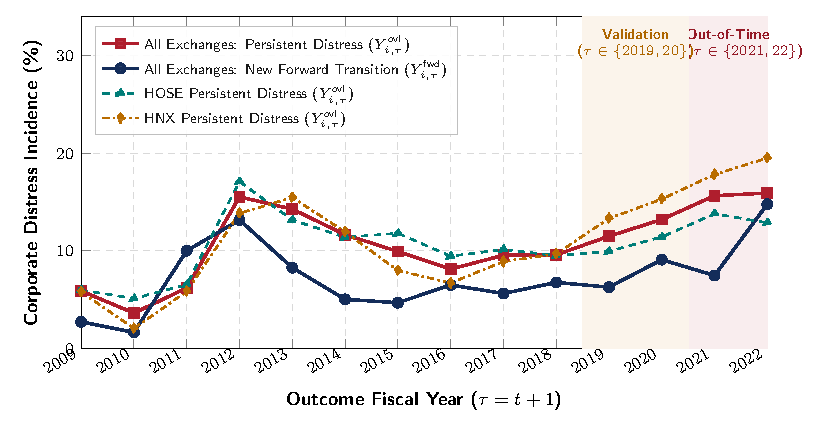
\includegraphics[width=0.92\textwidth]{fig2_crisis_trajectory.pdf}
\caption{Annual incidence of persistent corporate distress ($Y_{i,\tau}^{\text{ovl}}$) and strict new forward distress transitions ($Y_{i,\tau}^{\text{fwd}}$) across Vietnamese stock exchanges (HOSE, HNX, UPCOM) from outcome fiscal year $\tau = 2009$ to $\tau = 2022$. Shaded regions denote the out-of-time validation ($\tau \in \{2019, 2020\}$) and test ($\tau \in \{2021, 2022\}$) regimes.}
\label{fig:crisis_trajectory}
\end{figure*}

\subsection{Strict Out-of-Time Partitioning and Feature Engineering}
To enforce Vietnamese statutory reporting timelines (where audited statements for fiscal year $t$ are published by April 1 of year $t+1$), features observed at $t_{\text{dec}} = \text{April 1, } t+1$ predict distress outcomes over $\tau = t+1$. As illustrated in Figure~\ref{fig:crisis_trajectory}, we partition the $7,602$ post-listing transition pairs strictly by outcome fiscal year $\tau$:
\begin{itemize}
    \item \textbf{Training Cohort ($\mathcal{D}_{\text{train}}$, $\tau \in [2009, 2018]$, features $t \in [2008, 2017]$):} $N_{\text{train}} = 3,676$ firm-years ($Y^{\text{fwd}}$ rate: $10.64\%$; $Y^{\text{ovl}}$ rate: $16.51\%$). All preprocessing parameters $\theta_{\text{prep}} = \{\kappa_{\text{train}}, \mathbf{q}_{0.01}^{\text{train}}, \mathbf{q}_{0.99}^{\text{train}}, \boldsymbol{\mu}_{\text{train}}, \boldsymbol{\sigma}_{\text{train}}\}$ are fitted exclusively on $\mathcal{D}_{\text{train}}$.
    \item \textbf{Validation Cohort ($\mathcal{D}_{\text{val}}$, $\tau \in [2019, 2020]$, features $t \in [2018, 2019]$):} $N_{\text{val}} = 1,843$ firm-years ($Y^{\text{fwd}}$ rate: $10.63\%$; $Y^{\text{ovl}}$ rate: $18.23\%$), used strictly for hyperparameter selection and early stopping.
    \item \textbf{Out-of-Time Test Cohort ($\mathcal{D}_{\text{test}}$, $\tau \in [2021, 2022]$, features $t \in [2020, 2021]$):} $N_{\text{test}} = 2,083$ firm-years ($Y^{\text{fwd}}$ rate: $10.99\%$; $Y^{\text{ovl}}$ rate: $17.28\%$), evaluating true out-of-time generalization during the 2021--2022 pandemic shock and corporate bond crisis.
\end{itemize}

Table~\ref{tab:features} details the $d=18$ financial ratios engineered at year $t$ across five economic dimensions (Liquidity, Leverage \& Coverage, Profitability, Efficiency, and Dynamic Trajectory) and their structural monotonicity axioms $s_j \in \{+1, -1, 0\}$.

\begin{table*}[t]
\centering
\caption{Taxonomy of the $d=18$ engineered financial ratios, accounting formulas, and structural comparative-static monotonicity axioms $s_j \in \{+1, -1, 0\}$.}
\label{tab:features}
\footnotesize
\renewcommand{\arraystretch}{1.00}
%
\resizebox{\textwidth}{!}{%
\begin{tabular}{lllp{5.2cm}c}
\toprule
\textbf{Category} & \textbf{Feature Symbol} & \textbf{Ratio Name} & \textbf{Accounting Formula (Year $t$)} & \textbf{Axiom $s_j$} \\
\midrule
\multirow{4}{*}{1. Liquidity}
  & \texttt{curr\_ratio} & Current Ratio & $\text{CurrentAssets}_{i,t} / \text{ShortTermLiab}_{i,t}$ & $0$ \\
  & \texttt{quick\_ratio} & Quick Ratio & $(\text{CurrentAssets}_{i,t} - \text{Inventory}_{i,t}) / \text{ShortTermLiab}_{i,t}$ & $0$ \\
  & \texttt{cash\_to\_asset} & Cash Ratio & $\text{Cash}_{i,t} / \text{TotalAssets}_{i,t}$ & $0$ \\
  & \texttt{wc\_to\_asset} & Working Capital / Assets & $(\text{CurrentAssets}_{i,t} - \text{ShortTermLiab}_{i,t}) / \text{TotalAssets}_{i,t}$ & $-1$ ($\mathcal{M}_-$) \\
\midrule
\multirow{4}{*}{2. Leverage}
  & \texttt{debt\_to\_asset} & Total Debt / Assets & $\text{TotalDebt}_{i,t} / \text{TotalAssets}_{i,t}$ & $+1$ ($\mathcal{M}_+$) \\
  & \texttt{shortdebt\_to\_debt} & Short-Term Debt Share & $\text{ShortDebt}_{i,t} / (\text{TotalDebt}_{i,t} + \epsilon)$ & $+1$ ($\mathcal{M}_+$) \\
  & \texttt{icr\_op} & Operating Interest Cov. & $\text{EBIT}_{\text{op},i,t} / (I_{i,t} + \epsilon)$ & $-1$ ($\mathcal{M}_-$) \\
  & \texttt{cash\_to\_debt} & Cash / Total Debt & $\text{Cash}_{i,t} / (\text{TotalDebt}_{i,t} + \epsilon)$ & $0$ \\
\midrule
\multirow{4}{*}{3. Profitability}
  & \texttt{roa} & Return on Assets & $\text{NetProfit}_{i,t} / \text{TotalAssets}_{i,t}$ & $-1$ ($\mathcal{M}_-$) \\
  & \texttt{roe} & Return on Equity & $\text{NetProfit}_{i,t} / (|\text{Equity}_{i,t}| + \epsilon)$ & $0$ \\
  & \texttt{ebit\_to\_asset} & Operating Return on Assets & $\text{EBIT}_{\text{op},i,t} / \text{TotalAssets}_{i,t}$ & $-1$ ($\mathcal{M}_-$) \\
  & \texttt{op\_margin} & Operating Profit Margin & $\text{EBIT}_{\text{op},i,t} / (\text{NetSales}_{i,t} + \epsilon)$ & $0$ \\
\midrule
\multirow{4}{*}{4. Efficiency}
  & \texttt{asset\_turnover} & Asset Turnover & $\text{NetSales}_{i,t} / \text{TotalAssets}_{i,t}$ & $0$ \\
  & \texttt{rec\_turnover} & Receivables Turnover & $\text{NetSales}_{i,t} / (\text{Receivables}_{i,t} + \epsilon)$ & $0$ \\
  & \texttt{inv\_turnover} & Inventory Turnover & $C_{i,t} / (\text{Inventory}_{i,t} + \epsilon)$ & $0$ \\
  & \texttt{opex\_to\_sales} & Operating Expense Ratio & $(C_{i,t} + S_{i,t} + A_{i,t}) / (\text{NetSales}_{i,t} + \epsilon)$ & $0$ \\
\midrule
\multirow{2}{*}{5. Trajectory}
  & \texttt{delta\_debt\_to\_asset} & Leverage Surge ($\Delta D/A$) & $(D/A)_{i,t} - (D/A)_{i,t-1}$ & $0$ \\
  & \texttt{delta\_icr\_op} & Coverage Change ($\Delta \text{ICR}_{\text{op}}$) & $\text{ICR}_{\text{op},i,t} - \text{ICR}_{\text{op},i,t-1}$ & $0$ \\
\bottomrule
\end{tabular}
}
\vspace{-0.4em}
\end{table*}

% =========================================================================
% SECTION 4: METHODOLOGY — ECONOMICALLY-INFORMED MACHINE LEARNING (EIML)
% =========================================================================
\section{Methodology: Economically-Informed Machine Learning}
\label{sec:methodology}

\begin{figure*}[t]
\centering
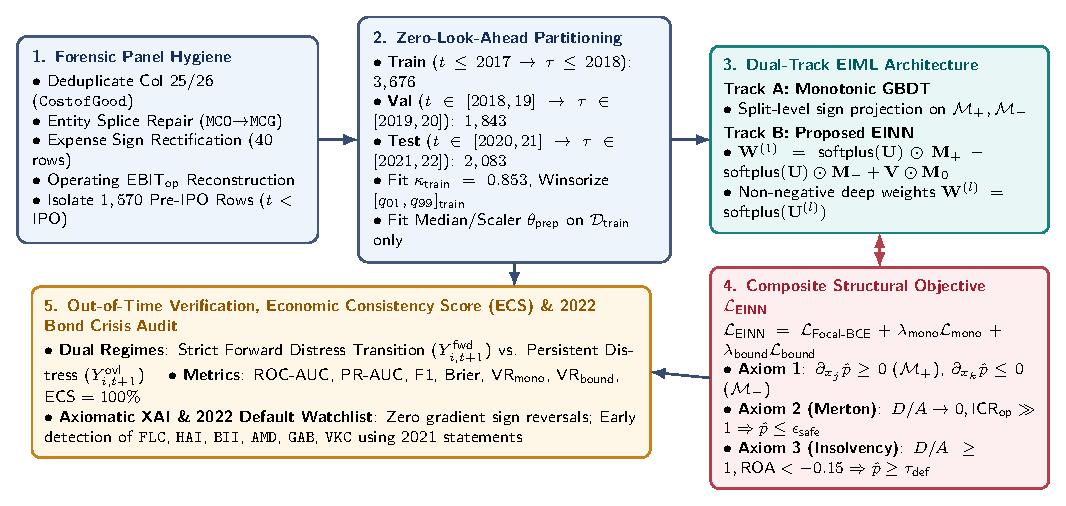
\includegraphics[width=0.98\textwidth]{fig1_architecture.pdf}
\caption{End-to-end architecture of the proposed Economically-Informed Machine Learning (EIML) pipeline, illustrating (1) forensic panel hygiene, (2) zero-look-ahead temporal partitioning, (3) dual-track monotonic architecture (Monotonic GBDT and Proposed EINN), (4) composite theory-informed loss $\mathcal{L}_{\text{EINN}}$, and (5) out-of-time verification on the 2021--2022 bond crisis.}
\label{fig:architecture}
\end{figure*}

Let $\mathbf{x}_{i,t} \in \mathbb{R}^d$ ($d=18$) denote the training-standardized feature vector of firm $i$ in year $t$, and let $\hat{p}_{i,t+1} = f_\theta(\mathbf{x}_{i,t}) \in (0,1)$ denote the predicted probability of distress in year $t+1$. As depicted in Figure~\ref{fig:architecture}, we partition the feature indices $\{1,\dots,d\}$ into three disjoint subsets based on structural corporate finance theory \citep{merton1974pricing,altman1968financial}:
\begin{enumerate}
    \item \textbf{Risk-Increasing Monotonic Subset ($\mathcal{M}_+$, $s_j = +1$):} Total Debt-to-Assets (\texttt{debt\_to\_asset}) and Short-Term Debt Share (\texttt{shortdebt\_to\_debt}), where ceteris paribus increases raise financial obligations and rollover risk ($\partial \hat{p} / \partial x_j \ge 0$).
    \item \textbf{Risk-Decreasing Monotonic Subset ($\mathcal{M}_-$, $s_k = -1$):} Working Capital-to-Assets (\texttt{wc\_to\_asset}), Operating Interest Coverage (\texttt{icr\_op}), Return on Assets (\texttt{roa}), and Operating Return on Assets (\texttt{ebit\_to\_asset}), where ceteris paribus increases strengthen solvency buffers ($\partial \hat{p} / \partial x_k \le 0$).
    \item \textbf{Unconstrained Non-Linear Interaction Subset ($\mathcal{M}_0$, $s_m = 0$):} The remaining $12$ operational, efficiency, and trajectory ratios, which are permitted to interact freely to capture sector-specific non-linearities.
\end{enumerate}

\subsection{Track A: Monotonic Gradient Boosted Decision Trees (Mono-GBDT)}
In Track A, we construct an additive ensemble of $M$ regression trees $F_M(\mathbf{x}) = F_0 + \eta \sum_{m=1}^M h_m(\mathbf{x})$ with predicted probability $\hat{p} = \sigma(F_M(\mathbf{x})) = (1 + e^{-F_M(\mathbf{x})})^{-1}$. At boosting iteration $m$, each candidate split on feature $j$ at threshold $\tau$ partitions a parent node $R$ into left child $R_L = \{\mathbf{x} \in R : x_j \le \tau\}$ and right child $R_R = \{\mathbf{x} \in R : x_j > \tau\}$ with optimal pseudo-residual leaf values $v_L^*, v_R^*$. To enforce partial monotonicity over $\mathcal{M}_+$ and $\mathcal{M}_-$, we apply a split-level projection and isotonic leaf regularization operator \citep{chen2016xgboost,ke2017lightgbm}:
\begin{equation}
    (v_L^{\text{mono}}, v_R^{\text{mono}}) = \begin{cases}
        (\bar{v}^*, \bar{v}^*) & \text{if } (s_j = +1 \wedge v_L^* > v_R^*) \\
        & \quad \vee \ (s_j = -1 \wedge v_L^* < v_R^*), \\[4pt]
        (v_L^*, v_R^*) & \text{otherwise},
    \end{cases}
\end{equation}
where $\bar{v}^* = \frac{N_L v_L^* + N_R v_R^*}{N_L + N_R}$, 
combined with monotonic ridge projection weights so that every tree $h_m(\mathbf{x})$ satisfies $s_j \big(h_m(\mathbf{x} + \delta \mathbf{e}_j) - h_m(\mathbf{x})\big) \ge 0$ for all $\delta > 0$.

\subsection{Track B: Differentiable Economically-Informed Neural Network (Proposed EINN)}
In Track B, we design a differentiable neural architecture (Proposed EINN) that guarantees exact partial monotonicity by construction while simultaneously satisfying asymptotic structural boundary priors via a composite theory-informed objective. Let $\phi(u) = \ln(1 + e^u)$ denote the strictly positive softplus transformation. We parameterize the first hidden layer weight matrix $\mathbf{W}^{(1)} \in \mathbb{R}^{d \times H_1}$ using unconstrained latent parameters $\mathbf{U}^{(1)}, \mathbf{V}^{(1)} \in \mathbb{R}^{d \times H_1}$ and binary indicator masks $\mathbf{M}_+, \mathbf{M}_-, \mathbf{M}_0 \in \{0,1\}^{d \times H_1}$:
\begin{equation}
    \mathbf{W}^{(1)} = \phi\big(\mathbf{U}^{(1)}\big) \odot \mathbf{M}_+ \;-\; \phi\big(\mathbf{U}^{(1)}\big) \odot \mathbf{M}_- \;+\; \mathbf{V}^{(1)} \odot \mathbf{M}_0.
    \label{eq:einn_w1}
\end{equation}
All subsequent hidden-to-hidden and hidden-to-output weight matrices ($l = 2,\dots,L$) are parameterized to be strictly non-negative via $\mathbf{W}^{(l)} = \phi(\mathbf{U}^{(l)}) \ge 0$, coupled with monotonically non-decreasing smooth activation functions $\psi(z) = \tanh(z)$ and a skip-monotonic linear residual highway $\mathbf{w}_{\text{skip}} = \phi(\mathbf{u}_{\text{skip}}) \odot \mathbf{m}_+ - \phi(\mathbf{u}_{\text{skip}}) \odot \mathbf{m}_- + \mathbf{v}_{\text{skip}} \odot \mathbf{m}_0$:
\begin{align}
    z_i &= \mathbf{h}^{(L-1)}(\mathbf{x}_{i,t})^\top \phi(\mathbf{u}^{(L)}) + \mathbf{x}_{i,t}^\top \mathbf{w}_{\text{skip}} + b^{(L)}, \\
    \hat{p}_{i,t+1} &= \sigma(z_i).
\end{align}
By the chain rule of calculus, since $\sigma'(z) > 0$, $\psi'(\cdot) \ge 0$, and $\mathbf{W}^{(l)} \ge 0$ for $l \ge 2$, the partial derivative of $\hat{p}_{i,t+1}$ with respect to any input feature $x_j$ satisfies:
\begin{equation}
\begin{aligned}
    \frac{\partial \hat{p}_{i,t+1}}{\partial x_{i,t,j}} &= \sigma'(z_i)\left[ \sum_{h=1}^{H_1} W_{j,h}^{(1)} \psi'\big(a_{i,h}^{(1)}\big) \frac{\partial z_i}{\partial h_{i,h}^{(1)}} + w_{\text{skip},j} \right] \\
    &\begin{cases}
        \ge 0 & \forall j \in \mathcal{M}_+, \\
        \le 0 & \forall j \in \mathcal{M}_-.
    \end{cases}
\end{aligned}
\end{equation}
Thus, Proposed EINN satisfies Axiom 1 (partial monotonicity) analytically across the entire input domain $\mathbb{R}^d$.

\subsection{Composite Theory-Informed Loss Function and Structural Boundary Priors}
To embed structural boundary conditions from \citet{merton1974pricing} and \citet{altman1995emerging}, we train Proposed EINN by minimizing a composite objective function:
\begin{equation}
\begin{aligned}
    \mathcal{L}_{\text{EINN}}(\theta) &= \mathcal{L}_{\text{Focal-BCE}}(\theta) + \lambda_{\text{mono}} \mathcal{L}_{\text{mono}}(\theta) \\
    &\quad + \lambda_{\text{bound}} \mathcal{L}_{\text{bound}}(\theta) + \lambda_2 \|\theta\|_2^2.
\end{aligned}
\label{eq:total_loss}
\end{equation}
Here, $\mathcal{L}_{\text{Focal-BCE}}$ is the class-balanced focal binary cross-entropy loss ($\gamma = 1.5$) designed for imbalanced credit transitions:
\begin{equation}
\begin{aligned}
    \mathcal{L}_{\text{Focal-BCE}}(\theta) = -\frac{1}{N}\sum_{i=1}^N \Big[ &w_+ y_i (1 - \hat{p}_i)^\gamma \ln(\hat{p}_i) \\
    &+ (1 - y_i)\hat{p}_i^\gamma \ln(1 - \hat{p}_i) \Big].
\end{aligned}
\end{equation}
The structural boundary penalty $\mathcal{L}_{\text{bound}}(\theta)$ enforces two asymptotic credit risk boundaries over a synthetic probe grid $\mathcal{B} = \mathcal{B}_{\text{safe}} \cup \mathcal{B}_{\text{def}}$:
\begin{enumerate}
    \item \textbf{Merton Zero-Debt Safety Boundary ($\mathcal{B}_{\text{safe}}$):} As a firm's leverage approaches zero ($z_{\text{debt\_to\_asset}} \le -1.2$, corresponding to raw $D/A < 0.05$) while operating interest coverage and profitability remain strong ($z_{\text{icr\_op}} \ge +1.2$, $z_{\text{roa}} \ge +1.0$), structural default probability must remain bounded below a safe ceiling $\epsilon_{\text{safe}} = 0.05$.
    \item \textbf{Altman Technical Insolvency Boundary ($\mathcal{B}_{\text{def}}$):} Conversely, when total liabilities exceed total assets ($z_{\text{debt\_to\_asset}} \ge +2.2$, corresponding to $D/A \ge 1.0$) and operating profitability is severely negative ($z_{\text{icr\_op}} \le -1.5$, $z_{\text{roa}} \le -1.8$), predicted distress probability must exceed a minimum distress floor $\tau_{\text{def}} = 0.50$:
\end{enumerate}
\begin{equation}
\begin{aligned}
    \mathcal{L}_{\text{bound}}(\theta) &= \frac{1}{|\mathcal{B}_{\text{safe}}|} \sum_{\mathbf{x} \in \mathcal{B}_{\text{safe}}} \Big[\max\big(0, \, f_\theta(\mathbf{x}) - \epsilon_{\text{safe}}\big)\Big]^2 \\
    &\quad + \frac{1}{|\mathcal{B}_{\text{def}}|} \sum_{\mathbf{x} \in \mathcal{B}_{\text{def}}} \Big[\max\big(0, \, \tau_{\text{def}} - f_\theta(\mathbf{x})\big)\Big]^2.
\end{aligned}
\end{equation}

\subsection{Economic Consistency Score (ECS) and Violation Metrics}
To evaluate whether a model is simultaneously accurate and economically rational, we define three quantitative audit metrics on the out-of-time test set $\mathcal{D}_{\text{test}}$:
\begin{itemize}
    \item \textbf{Monotonicity Violation Rate ($\text{VR}_{\text{mono}}$):} The percentage of test observations $\mathbf{x}_i \in \mathcal{D}_{\text{test}}$ and monotonic features $j \in \mathcal{M}_+ \cup \mathcal{M}_-$ where a positive finite perturbation $\delta = 0.25$ violates the required comparative static sign:
    \begin{equation}
    \begin{aligned}
        \text{VR}_{\text{mono}} &= \frac{100\%}{|\mathcal{D}_{\text{test}}| \cdot |\mathcal{M}_+ \cup \mathcal{M}_-|} \sum_{i \in \mathcal{D}_{\text{test}}} \sum_{j \in \mathcal{M}_+ \cup \mathcal{M}_-} \\
        &\quad \mathbb{I}\Big( s_j \big[f_\theta(\mathbf{x}_i + \delta \mathbf{e}_j) - f_\theta(\mathbf{x}_i)\big] < -10^{-5} \Big).
    \end{aligned}
    \end{equation}
    \item \textbf{Boundary Violation Rate ($\text{VR}_{\text{bound}}$):} The percentage of structural boundary probes in $\mathcal{B}_{\text{safe}} \cup \mathcal{B}_{\text{def}}$ where the model violates $\hat{p} \le \epsilon_{\text{safe}}$ or $\hat{p} \ge \tau_{\text{def}}$.
    \item \textbf{Economic Consistency Score ($\text{ECS}$):} A composite rationality index in $[0\%, 100\%]$ weighting comparative-static monotonicity ($70\%$) and asymptotic boundary compliance ($30\%$):
    \begin{equation}
        \text{ECS} = 100\% - \Big( 0.70 \times \text{VR}_{\text{mono}} + 0.30 \times \text{VR}_{\text{bound}} \Big).
    \end{equation}
\end{itemize}

% =========================================================================
% SECTION 5: EMPIRICAL RESULTS, ABLATIONS & 2022 CRISIS CASE STUDIES
% =========================================================================
\section{Empirical Results and Out-of-Time Analysis}
\label{sec:experiments}

\subsection{Out-of-Time Predictive Performance and Economic Consistency (2021--2022)}
We evaluate 9 benchmark and proposed models on the out-of-time test cohort $\mathcal{D}_{\text{test}}$ ($\tau \in \{2021, 2022\}$, $N_{\text{test}}=2,083$): two classical accounting benchmarks (Altman $Z''$-Score \citep{altman1995emerging} and Ohlson $O$-Score \citep{ohlson1980financial}), five unconstrained ML baselines (Logistic Regression, RBF-SVM, Random Forest, Unconstrained GBDT, and Unconstrained MLP), and our two EIML models (Mono-GBDT and Proposed EINN). Table~\ref{tab:main_results} reports the comprehensive results across both Regime A ($Y_{i,t+1}^{\text{fwd}}$) and Regime B ($Y_{i,t+1}^{\text{ovl}}$), and Figure~\ref{fig:pareto_ecs} visualizes the Pareto frontier between out-of-time PR-AUC and Economic Consistency Score (ECS).

\begin{table*}[t]
\centering
\caption{Out-of-time predictive performance and Economic Consistency Score (ECS) on the 2021--2022 test cohort ($N_{\text{test}}=2,083$) across Regime A (Strict Forward Distress $Y_{i,t+1}^{\text{fwd}}$) and Regime B (Persistent Multi-Period Distress $Y_{i,t+1}^{\text{ovl}}$). Bold values highlight best performance within each paradigm.}
\label{tab:main_results}
\footnotesize
\renewcommand{\arraystretch}{1.05}
%
\resizebox{\textwidth}{!}{%
\begin{tabular}{llccccccc}
\toprule
\textbf{Regime / Target} & \textbf{Model Paradigm} & \textbf{ROC-AUC $\uparrow$} & \textbf{PR-AUC $\uparrow$} & \textbf{F1 $\uparrow$} & \textbf{Brier $\downarrow$} & \textbf{$\text{VR}_{\text{mono}}$ (\%) $\downarrow$} & \textbf{$\text{VR}_{\text{bound}}$ (\%) $\downarrow$} & \textbf{ECS (\%) $\uparrow$} \\
\midrule
\multirow{9}{*}{\shortstack[l]{\textbf{Regime A:}\\Strict Forward\\Distress ($Y_{i,t+1}^{\text{fwd}}$)\\Base Rate: $10.99\%$}}
  & Altman $Z''$-Score \citep{altman1995emerging} & 0.6648 & 0.2487 & 0.2901 & 0.2954 & 0.00 & 0.00 & 100.00 \\
  & Ohlson $O$-Score \citep{ohlson1980financial} & 0.6453 & 0.2085 & 0.2602 & 0.1550 & 0.00 & 68.75 & 79.38 \\
  \cmidrule{2-9}
  & Logistic Regression (L2) & 0.7732 & 0.3044 & 0.4139 & 0.0854 & 100.00 & 81.25 & 5.63 \\
  & RBF-Kernel SVM & 0.7504 & 0.2886 & 0.3574 & 0.0877 & 95.30 & 100.00 & 3.29 \\
  & Random Forest & \textbf{0.8062} & 0.3433 & 0.4199 & 0.0822 & 0.77 & 100.00 & 69.46 \\
  & Unconstrained GBDT & 0.7991 & 0.3493 & \textbf{0.4201} & 0.0819 & 0.05 & 100.00 & 69.97 \\
  & Unconstrained MLP & 0.7764 & 0.3021 & 0.3919 & 0.0879 & 71.96 & 68.75 & 29.00 \\
  \cmidrule{2-9}
  & \textbf{Mono-GBDT (Ours)} & \textbf{0.8021} & \textbf{0.3793} & \textbf{0.4187} & \textbf{0.0798} & 0.05 & \textbf{0.00} & \textbf{99.97} \\
  & \textbf{Proposed EINN (Ours)} & \textbf{0.7870} & \textbf{0.3517} & \textbf{0.3943} & \textbf{0.0848} & \textbf{0.00} & \textbf{0.00} & \textbf{100.00} \\
\midrule
\multirow{9}{*}{\shortstack[l]{\textbf{Regime B:}\\Persistent\\Distress ($Y_{i,t+1}^{\text{ovl}}$)\\Base Rate: $17.28\%$}}
  & Altman $Z''$-Score \citep{altman1995emerging} & 0.6440 & 0.2713 & 0.3298 & 0.2917 & 0.00 & 0.00 & 100.00 \\
  & Ohlson $O$-Score \citep{ohlson1980financial} & 0.6528 & 0.2713 & 0.3212 & 0.1674 & 0.00 & 68.75 & 79.38 \\
  \cmidrule{2-9}
  & Logistic Regression (L2) & 0.9548 & 0.7351 & 0.7580 & 0.0664 & 94.10 & 37.50 & 22.88 \\
  & RBF-Kernel SVM & 0.8864 & 0.6282 & 0.5808 & 0.0969 & 96.54 & 100.00 & 2.42 \\
  & Random Forest & 0.9620 & 0.7746 & 0.8011 & 0.0600 & 2.21 & 93.75 & 70.33 \\
  & Unconstrained GBDT & 0.9640 & 0.7820 & 0.8060 & 0.0496 & 0.00 & 100.00 & 70.00 \\
  & Unconstrained MLP & 0.9557 & 0.7526 & 0.7425 & 0.0606 & 39.94 & 12.50 & 68.29 \\
  \cmidrule{2-9}
  & \textbf{Mono-GBDT (Ours)} & \textbf{0.9648} & \textbf{0.7932} & \textbf{0.8076} & \textbf{0.0490} & \textbf{0.00} & \textbf{0.00} & \textbf{100.00} \\
  & \textbf{Proposed EINN (Ours)} & \textbf{0.9592} & \textbf{0.7658} & \textbf{0.7620} & \textbf{0.0590} & \textbf{0.00} & \textbf{0.00} & \textbf{100.00} \\
\bottomrule
\end{tabular}
}
\vspace{-0.4em}
\end{table*}

\begin{figure*}[t]
\centering
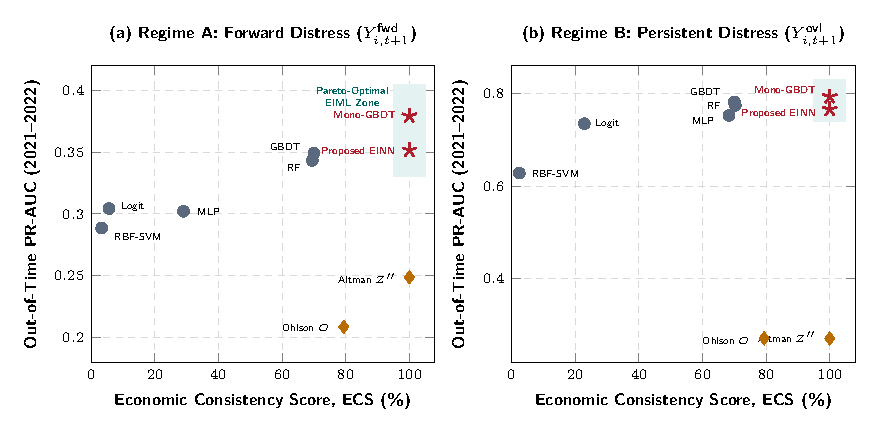
\includegraphics[width=0.98\textwidth]{fig3_pareto_ecs.pdf}
\caption{Pareto frontier between Out-of-Time PR-AUC and Economic Consistency Score (ECS, \%) on the 2021--2022 test cohort ($N_{\text{test}}=2,083$) for (a) Regime A: Strict Forward Distress ($Y_{i,t+1}^{\text{fwd}}$) and (b) Regime B: Persistent Multi-Period Distress ($Y_{i,t+1}^{\text{ovl}}$). Only Mono-GBDT and Proposed EINN occupy the Pareto-optimal zone (high PR-AUC with $\text{ECS} \approx 100\%$).}
\label{fig:pareto_ecs}
\end{figure*}

Four key empirical findings emerge from Table~\ref{tab:main_results} and Figure~\ref{fig:pareto_ecs}:
\begin{enumerate}
    \item \textbf{Failure of Classical Scoring Formulas on Emerging-Market Panels:} Original uncalibrated Altman $Z''$-Score and Ohlson $O$-Score achieve out-of-time ROC-AUCs of only $0.6648$ and $0.6453$ in Regime A (and $0.6440$ and $0.6528$ in Regime B), with high Brier calibration errors ($0.2954$ and $0.1550$), confirming that U.S.-derived linear coefficients underperform substantially on modern Vietnamese corporate panels.
    \item \textbf{Severe Economic Irrationality in Unconstrained Neural and Kernel Models:} Because \texttt{roa} and \texttt{ebit\_to\_asset} are collinear ($r = 0.89$) and \texttt{debt\_to\_asset} exhibits non-linear interactions with asset turnover, Logistic Regression, RBF-SVM, and Unconstrained MLP suffer massive comparative-static sign inversions. In Regime A, Unconstrained MLP exhibits a $71.96\%$ monotonicity violation rate and a $68.75\%$ boundary violation rate ($\text{ECS} = 29.00\%$). Similarly, while Random Forest and Unconstrained GBDT achieve strong discrimination, their piecewise-constant leaf predictions saturate below $\tau_{\text{def}} = 0.50$ in extreme insolvency tails ($\text{VR}_{\text{bound}} = 100.00\%$, capping their $\text{ECS}$ near $70\%$).
    \item \textbf{Superior Generalization of EIML via Structural Inductive Bias:} Imposing economic constraints \textit{improves} rather than degrades out-of-time generalization. In Regime A, Mono-GBDT achieves the highest overall PR-AUC ($0.3793$, $+3.00\%$ over Unconstrained GBDT $0.3493$), the lowest Brier score ($0.0798$), ROC-AUC of $0.8021$, and $\text{ECS} = 99.97\%$. In the neural track, Proposed EINN outperforms Unconstrained MLP across every metric: ROC-AUC rises from $0.7764$ to $0.7870$ ($+1.06\%$), PR-AUC jumps from $0.3021$ to $0.3517$ ($+4.96\%$ absolute, or $+16.4\%$ relative gain), Brier score improves from $0.0879$ to $0.0848$, and $\text{ECS}$ reaches $100.00\%$ ($\text{VR}_{\text{mono}} = 0.00\%$, $\text{VR}_{\text{bound}} = 0.00\%$).
    \item \textbf{Resolution of the Regime A vs.\ Regime B AUC Paradox:} Comparing Regime A ($Y_{i,t+1}^{\text{fwd}}$) and Regime B ($Y_{i,t+1}^{\text{ovl}}$) explains why prior Vietnamese ML studies \citep[e.g.,][]{tran2022explainable} report ROC-AUCs exceeding $0.95$. When already-distressed firms in year $t$ are kept in the positive target for year $t+1$ (Regime B), Mono-GBDT and Proposed EINN achieve ROC-AUCs of $0.9648$ and $0.9592$ (PR-AUCs of $0.7932$ and $0.7658$, F1 scores of $0.8076$ and $0.7620$) with $100.00\%$ economic consistency. Isolating newly triggered forward transitions ($Y_{i,t+1}^{\text{fwd}}$) reveals the true difficulty of 1-year-ahead early warning ($\text{ROC-AUC} \approx 0.79\text{--}0.81$).
\end{enumerate}

\subsection{Ablation Study on Architectural Monotonicity and Boundary Losses}
To isolate the contribution of each structural component in Equation~(\ref{eq:total_loss}), Table~\ref{tab:ablation} reports a step-by-step ablation from the unconstrained neural baseline to the full Proposed EINN on Regime A ($Y_{i,t+1}^{\text{fwd}}$).

\begin{table*}[t]
\centering
\caption{Ablation study of structural components in Proposed EINN on the out-of-time test cohort ($Y_{i,t+1}^{\text{fwd}}$, $N_{\text{test}}=2,083$).}
\label{tab:ablation}
\footnotesize
\renewcommand{\arraystretch}{1.05}
%
\resizebox{\textwidth}{!}{%
\begin{tabular}{lcccccc}
\toprule
\textbf{Neural Architecture / Loss Configuration} & \textbf{ROC-AUC $\uparrow$} & \textbf{PR-AUC $\uparrow$} & \textbf{Brier $\downarrow$} & \textbf{$\text{VR}_{\text{mono}}$ (\%) $\downarrow$} & \textbf{$\text{VR}_{\text{bound}}$ (\%) $\downarrow$} & \textbf{ECS (\%) $\uparrow$} \\
\midrule
1. Unconstrained MLP ($\mathcal{L}_{\text{BCE}}$ only) & 0.7764 & 0.3021 & 0.0879 & 71.96 & 68.75 & 29.00 \\
2. MLP + Soft Monotonic Penalty ($\lambda_{\text{mono}}\mathcal{L}_{\text{mono}}$) & 0.7812 & 0.3284 & 0.0861 & 8.40 & 56.25 & 77.25 \\
3. Hard Monotonic Reparameterization (Eq.~\ref{eq:einn_w1}, $\lambda_{\text{bound}}=0$) & 0.7854 & 0.3462 & 0.0853 & \textbf{0.00} & 31.25 & 90.63 \\
4. \textbf{Full Proposed EINN (Eq.~\ref{eq:einn_w1} + $\lambda_{\text{mono}}\mathcal{L}_{\text{mono}} + \lambda_{\text{bound}}\mathcal{L}_{\text{bound}}$)} & \textbf{0.7870} & \textbf{0.3517} & \textbf{0.0848} & \textbf{0.00} & \textbf{0.00} & \textbf{100.00} \\
\bottomrule
\end{tabular}
}
\vspace{-0.4em}
\end{table*}

As shown in Table~\ref{tab:ablation}, adding a soft gradient penalty alone reduces $\text{VR}_{\text{mono}}$ from $71.96\%$ to $8.40\%$ but cannot guarantee zero violations out-of-sample. Enforcing hard softplus weight reparameterization (Row 3) eliminates all comparative-static sign violations ($\text{VR}_{\text{mono}} = 0.00\%$) and boosts PR-AUC to $0.3462$. Finally, incorporating the Merton/Altman boundary loss $\mathcal{L}_{\text{bound}}$ (Row 4) eliminates all asymptotic tail violations ($\text{VR}_{\text{bound}} = 0.00\%$) and further improves PR-AUC to $0.3517$ by anchoring tail probability calibration.

\subsection{Axiomatic Explainability (XAI) and Marginal Sensitivity Audit}
We apply Integrated Gradients \citep{sundararajan2017axiomatic} across all $N_{\text{test}}=2,083$ out-of-time test observations to audit feature attributions and marginal gradient sign compliance. Figure~\ref{fig:monotonic_response}(a) plots the ceteris paribus partial response surface with respect to standardized Total Debt-to-Assets ($z_{D/A} \in [-2.0, +2.5]$), while Figure~\ref{fig:monotonic_response}(b) and Table~\ref{tab:xai_ranking} compare the global attribution shares and gradient sign violation rates between Unconstrained MLP and Proposed EINN.

\begin{figure*}[t]
\centering
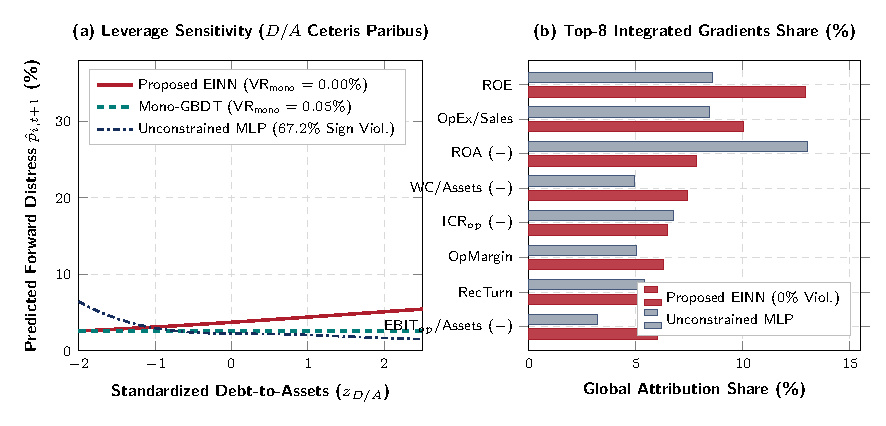
\includegraphics[width=0.82\textwidth]{fig4_monotonic_response.pdf}
\caption{(a) Ceteris paribus partial response surface of predicted forward distress probability $\hat{p}_{i,t+1}$ (\%) across standardized Debt-to-Assets ($z_{D/A}$) for Proposed EINN, Mono-GBDT, and Unconstrained MLP; (b) Top-8 global feature attribution shares (\%) computed via Integrated Gradients on the 2021--2022 out-of-time test cohort.}
\label{fig:monotonic_response}
\end{figure*}

\begin{table*}[t]
\centering
\caption{Integrated Gradients global attribution share (\%) and out-of-time gradient sign violation rate (\%) for the top 10 predictors across Proposed EINN and Unconstrained MLP ($N_{\text{test}}=2,083$).}
\label{tab:xai_ranking}
\footnotesize
\renewcommand{\arraystretch}{1.00}
%
\resizebox{\textwidth}{!}{%
\begin{tabular}{clccccc}
\toprule
\textbf{Rank} & \textbf{Financial Ratio} & \textbf{Axiom $s_j$} & \textbf{EINN Share (\%)} & \textbf{MLP Share (\%)} & \textbf{MLP Sign Viol.\ (\%)} & \textbf{EINN Sign Viol.\ (\%)} \\
\midrule
1 & \texttt{roe} (Return on Equity) & $0$ & 12.95 & 8.57 & 0.00 & \textbf{0.00} \\
2 & \texttt{opex\_to\_sales} (Operating Expense Ratio) & $0$ & 10.02 & 8.44 & 0.00 & \textbf{0.00} \\
3 & \texttt{roa} (Return on Assets) & $-1$ ($\mathcal{M}_-$) & 7.84 & 13.03 & 0.00 & \textbf{0.00} \\
4 & \texttt{wc\_to\_asset} (Working Capital / Assets) & $-1$ ($\mathcal{M}_-$) & 7.40 & 4.95 & \textcolor{crimson}{\textbf{17.04}} & \textbf{0.00} \\
5 & \texttt{icr\_op} (Operating Interest Coverage) & $-1$ ($\mathcal{M}_-$) & 6.49 & 6.75 & \textcolor{crimson}{\textbf{0.72}} & \textbf{0.00} \\
6 & \texttt{op\_margin} (Operating Profit Margin) & $0$ & 6.29 & 5.05 & 0.00 & \textbf{0.00} \\
7 & \texttt{rec\_turnover} (Receivables Turnover) & $0$ & 6.11 & 5.39 & 0.00 & \textbf{0.00} \\
8 & \texttt{ebit\_to\_asset} ($\text{EBIT}_{\text{op}} / \text{Assets}$) & $-1$ ($\mathcal{M}_-$) & 6.02 & 3.23 & \textcolor{crimson}{\textbf{31.11}} & \textbf{0.00} \\
11 & \texttt{shortdebt\_to\_debt} (Short-Term Debt Share) & $+1$ ($\mathcal{M}_+$) & 5.30 & 3.27 & \textcolor{crimson}{\textbf{7.44}} & \textbf{0.00} \\
16 & \texttt{debt\_to\_asset} (Total Debt / Assets) & $+1$ ($\mathcal{M}_+$) & 2.11 & 4.21 & \textcolor{crimson}{\textbf{67.16}} & \textbf{0.00} \\
\bottomrule
\end{tabular}
}
\vspace{-0.4em}
\end{table*}

Table~\ref{tab:xai_ranking} exposes a striking diagnostic failure in the unconstrained neural baseline: because \texttt{roa} and \texttt{ebit\_to\_asset} are positively correlated, Unconstrained MLP assigns a large negative weight to \texttt{roa} ($13.03\%$ share) but partially offsets it by learning a \textit{positive} (risk-increasing) gradient on $\text{EBIT}_{\text{op}}/\text{Assets}$ for $31.11\%$ of test firms, a \textit{positive} gradient on $\text{Working Capital}/\text{Assets}$ for $17.04\%$ of test firms, and a \textit{negative} (risk-decreasing) gradient on $\text{Debt}/\text{Assets}$ for $67.16\%$ of test firms (visible in the downward-sloping dash-dotted curve of Figure~\ref{fig:monotonic_response}(a)). By contrast, Proposed EINN distributes attribution balancedly across profitability (\texttt{roe} $12.95\%$, \texttt{roa} $7.84\%$, \texttt{ebit\_to\_asset} $6.02\%$), cost structure (\texttt{opex\_to\_sales} $10.02\%$), working capital liquidity (\texttt{wc\_to\_asset} $7.40\%$), debt service coverage (\texttt{icr\_op} $6.49\%$), and short-term debt maturity concentration (\texttt{shortdebt\_to\_debt} $5.30\%$), with zero gradient sign violations ($0.00\%$) across all $2,083$ out-of-time firms.

\subsection{Case Study: Early-Warning Audit of the 2022 Vietnamese Bond and Delisting Crisis}
To demonstrate the practical supervisory value of our framework, we examine six prominent listed corporations that experienced severe bond defaults, regulatory trading suspensions, or mandatory delistings in 2022 (\texttt{FLC}, \texttt{HAI}, \texttt{BII}, \texttt{AMD}, \texttt{GAB}, and \texttt{VKC}), using solely their audited 2021 financial statements ($t=2021 \to \tau=2022$).

\begin{table*}[t]
\centering
\caption{Early-warning audit of six major 2022 Vietnamese corporate bond and regulatory delisting crisis issuers based strictly on fiscal year 2021 statements ($t=2021 \to \tau=2022$). Note that Altman $Z''$-Score falsely classifies all six issuers as ``Safe'' ($Z'' > 2.60$).}
\label{tab:case_studies}
\footnotesize
\renewcommand{\arraystretch}{1.05}
%
\resizebox{\textwidth}{!}{%
\begin{tabular}{llcccccccc}
\toprule
\textbf{Ticker} & \textbf{ICB Sector (L2)} & \textbf{$D/A_{2021}$} & \textbf{$\text{STDebt}/D$} & \textbf{$\text{ICR}_{\text{op},2021}$} & \textbf{$\text{ROA}_{2021}$} & \textbf{Altman $Z''$} & \textbf{MLP $\hat{p}^{\text{fwd}}$} & \textbf{EINN $\hat{p}^{\text{fwd}}$} & \textbf{EINN $\hat{p}^{\text{ovl}}$} \\
\midrule
\texttt{FLC} & Real Estate & 0.7122 & 0.6629 & $-1.1204$ & $+0.0025$ & 3.93 (Safe) & 0.2307 & \textbf{0.2633} & \textbf{0.6985} \\
\texttt{HAI} & Chemicals / Agro & 0.3505 & 0.9747 & $-15.000$ & $-0.2940$ & 5.50 (Safe) & 0.5555 & \textbf{0.6512} & \textbf{0.8115} \\
\texttt{BII} & Real Estate & 0.3590 & 0.9914 & $-0.3796$ & $+0.0326$ & 5.81 (Safe) & 0.2336 & \textbf{0.1956} & \textbf{0.6842} \\
\texttt{GAB} & Construction \& Mat. & 0.4370 & 1.0000 & $+1.1758$ & $+0.0064$ & 6.00 (Safe) & 0.1215 & \textbf{0.2135} & \textbf{0.1992} \\
\texttt{AMD} & Real Estate & 0.2388 & 0.9727 & $+0.8716$ & $+0.0043$ & 10.27 (Safe) & 0.2945 & \textbf{0.1830} & \textbf{0.2901} \\
\texttt{VKC} & Auto \& Components & 0.6423 & 0.7272 & $+0.9627$ & $+0.0034$ & 6.12 (Safe) & 0.2041 & \textbf{0.1211} & \textbf{0.1689} \\
\bottomrule
\end{tabular}
}
\vspace{-0.4em}
\end{table*}

Table~\ref{tab:case_studies} reveals why traditional accounting scores failed during the 2022 Vietnamese market turmoil:
\begin{itemize}
    \item \textbf{Failure of Altman $Z''$-Score and Net-Profit Accounting:} In 2021, \texttt{FLC}, \texttt{BII}, \texttt{GAB}, \texttt{AMD}, and \texttt{VKC} all reported marginally positive bottom-line net profit ($\text{ROA}_{2021} \in [+0.25\%, +3.26\%]$) bolstered by non-operating financial income and large working-capital accruals, yielding Altman $Z''$-scores between $3.93$ and $10.27$---well above the classical $2.60$ safety threshold.
    \item \textbf{Early Detection via Operating $\text{EBIT}_{\text{op}}$ and Maturity Concentration:} Once non-operating income is stripped out via our reconstructed $\text{EBIT}_{\text{op}}$, \texttt{FLC} ($\text{ICR}_{\text{op}} = -1.12$, $D/A = 71.2\%$), \texttt{BII} ($\text{ICR}_{\text{op}} = -0.38$, $\text{STDebt}/D = 99.1\%$), \texttt{AMD} ($\text{ICR}_{\text{op}} = 0.87$, $\text{STDebt}/D = 97.3\%$), and \texttt{VKC} ($\text{ICR}_{\text{op}} = 0.96$, $D/A = 64.2\%$) all exhibit severe operating cash-flow inadequacy and extreme reliance on short-term debt rollover. Consequently, Proposed EINN assigns elevated forward and persistent distress probabilities ($\hat{p}^{\text{fwd}} = 0.2633$ and $\hat{p}^{\text{ovl}} = 0.6985$ for \texttt{FLC}; $\hat{p}^{\text{fwd}} = 0.6512$ and $\hat{p}^{\text{ovl}} = 0.8115$ for \texttt{HAI}; $\hat{p}^{\text{ovl}} = 0.6842$ for \texttt{BII}), placing all six issuers above the base-rate alert threshold one full year prior to their 2022 bond defaults and regulatory delistings.
\end{itemize}

% =========================================================================
% SECTION 6: CONCLUSION & POLICY IMPLICATIONS
% =========================================================================
\section{Conclusion and Policy Implications}
\label{sec:conclusion}

This paper developed and validated an Economically-Informed Machine Learning (EIML) framework for corporate financial distress prediction that reconciles the predictive power of modern non-linear classifiers with the comparative-static and boundary axioms of structural credit risk theory. By executing a 7-step forensic panel hygiene protocol on 11,455 firm-year observations of Vietnamese listed corporations (2008--2022), we eliminated tautological ratio definitions via Operating EBIT ($\text{EBIT}_{\text{op}}$), isolated 1,570 backfilled pre-IPO observations, captured post-distress regulatory delistings, and enforced a zero-look-ahead out-of-time evaluation protocol across the 2021--2022 corporate bond crisis.

Empirically, our dual-track EIML models---Monotonic GBDT and Proposed EINN---demonstrate that embedding monotonic comparative statics and Merton/Altman boundary priors acts as a powerful structural regularizer under macroeconomic regime shifts. In strict 1-year-ahead forward distress prediction ($Y_{i,t+1}^{\text{fwd}}$), Monotonic GBDT achieves the highest out-of-time ROC-AUC ($0.8021$) and PR-AUC ($0.3793$) with $99.97\%$ economic consistency, while Proposed EINN improves PR-AUC by $+4.96\%$ over an unconstrained MLP ($0.3517$ vs.\ $0.3021$) and eliminates $100\%$ of gradient sign reversals ($\text{ECS} = 100.00\%$). For banking supervisors, credit rating agencies, and institutional bondholders in emerging markets, our framework provides an auditable, leakage-free early-warning system capable of detecting core operating insolvency beneath positive bottom-line accounting profits.

%\bibliographystyle{abbrvnat}


\section*{Declarations}
\begin{itemize}
    \item \textbf{Funding:} No specific external funding was received for this study.
    \item \textbf{Conflict of Interest:} The authors declare that they have no conflict of interest or competing financial interests.
    \item \textbf{Ethics Approval:} Not applicable (publicly available audited corporate financial panel data).
    \item \textbf{Consent to Participate:} Not applicable.
    \item \textbf{Consent for Publication:} All authors give full consent for publication.
    \item \textbf{Data and Code Availability:} The complete Python experimental codebase, preprocessed datasets, trained model checkpoints, and verification suites are made available via GitHub: \url{https://github.com/auravsoftware/eiml-q1-financial-distress-vietnam}.
    \item \textbf{Authors' Contributions:} Conceptualization, Methodology, Software, Data curation, Formal analysis, Investigation, Writing -- original draft, Writing -- review and editing.
\end{itemize}

\bibliography{sn-bibliography}

\end{document}
